\chapter{Interface Application}
\label{interface_application}

    In this chapter, a detailed description of \emph{web application} will be made. Firstly, a general overview of application will be presented, followed by a more detailed explanation of \emph{client} and \emph{server} sides.

\section{Technology}

    \emph{Structs 2} was the chosen framework to implement the \emph{web application}. This is a very useful framework used to create MCV java web applications. Therefore, application is structured as follows:
    
    \underline{Views}:
    
    \begin{enumerate}
    \item \emph{index.jsp} - this is the initial view where all the calculation option are presented. The user is able to select one of the possible insulin calculation methods. After selected a given option, the input forms appears in the screen.
    \item \emph{meal\_personal.jsp} - in this method, the insulin sensitivity is calculated based on correlation between physical level and drop in blood sugar.
    \item \emph{meal\_standard} - similarly to the previous calculation method, all the parameters to needed to insulin calculation are requested to the user. However, in this case insulin sensitivity of the patient is explicitly indicated by him.
    \item \emph{background.jsp} - this view receives the patent's weight in order to calculate the background insulin dose.
    \item \emph{calculation\_results.jsp} - after all performed one of the considered insulin calculation method, this view presents the voted result. Additionally, the user can also check the results obtained in each web-service.
    
    
    
    \end{enumerate}
    
    \underline{Actions}:
    
    There is 3 distinct \emph{actions} to handle the each type of insulin dose calculation:
    
    \begin{enumerate}
    \item \emph{Background} - action called to calculate background insulin dose
    \item \emph{MealPersonal} - action called to firstly calculate patient's insulin sensitivity followed by insulin doses calculation.
    \item \emph{MealStandard} - action called to calculate background insulin dose based on a given insulin sensitivity
    \end{enumerate}
    
    All the considered actions are derived from a \emph{main action} named \textbf{User}. This action is responsible for the initialisation of a new \emph{bean} when it isn't already saved in the current session.
    
    \underline{Model}:
    
    Model is probably the most important part of this project. Web-services connections and voting system were implemented in this entity.
    
    There are 3 distinct main methods, one for each type of insulin dose calculation. Additionally, other methods were implemented to deal with web-service connections and voting system.

\section{Web Service Connection}

    In this section will be described the management of web-service connections and control of the service's response time.
    
    The first step consisted in implementing a new \emph{class}, named \emph{Client}, responsible for calling the web-service methods located at server-side. To call the web-service's methods an automatically generated \emph{proxy} was used, facilitating this task.
    
    Fig. \ref{FILHADAPUTA} shows an general overview of communication between \emph{model} and web-services. 
    
    \begin{figure}[H]
        \centering
        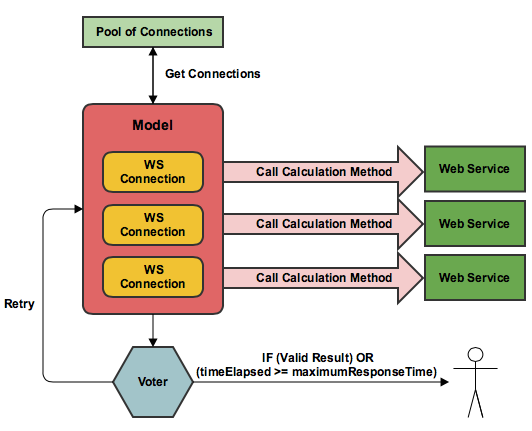
\includegraphics[width=\textwidth,height=\textheight,keepaspectratio]{webservice-2.png}
        \caption{Overview of communication between \emph{model} and web-services}
        \label{FILHADAPUTA}     
    \end{figure}
    
    Whenever the voter returns a valid result, the web-services used for the voting process are presented in the interface. Also the corresponded result of each one is shown.
    
\subsection{Pool of Connections}
    
    To manage the web-service's connections, a \emph{connections' pool} was implemented. This pool stores all the web-services URLs and allows the establishment of a new connection to a available web-service. So, when a \emph{model} method requires a new connection to a web-service, it calls the \emph{getNewConnection()} method from the pool of connections.
    
    Since a given web-service server can be offline, the pool stores a \emph{check-sum} indicating whether a given server is available or not. Note that a new connection corresponds to a new instance of \emph{Client} class.

\subsection{Limited Response Time}

    As requested, the user should receive the calculation result within a maximum period of 4 seconds. Therefore, some control mechanism were implemented to fulfil this requirement.
    
    The most trivial approach consisted in execute each request sequentially and setting an appropriate \emph{connection timeout} and \emph{request timeout} in web-service client. So a \emph{timeout exception} would be thrown by web-service client and that result will be not valid. However, some problems arises when using this approach. Thus, a different approach and possibly more elegant approach was adopted for this application.
    
    Firstly, all the web-services requests are running in parallel, meaning that each web-service's request is executed in an independent \emph{thread}. A \emph{maximum execution time} of each thread is defined being cancelled all the tasks that didn't finish within that time. When task doesn't finish, the result of that web-service is set with value -1, indicating that a \emph{timeout} occurred.
    
    However, when a given set of results are not enough to produce a valid result, the system establishes new connections and repeat the process while the elapsed time is less than 4 seconds.
    
\subsection{Error Handling}

    As described previously, a lot of exceptions can be thrown during a request of insulin calculation. To improve the robustness of the application, all the exceptions should be handled and notified to the user.
    
    The most important exceptions are related to the \emph{web-services' connections}. An exception is thrown whenever a given request thread could not achieve a valid result from the web-service. In this case, a new set of connections are established and the requests are performed again. However, when the elapsed time since user's request exceeds 4 seconds, the user is notified that something wrong happened.
    
    In order to simplify the error handling, when something wrong happens during a request the result is defined as -1. Thus, the user is redirected to the index page whenever a result equals to -1 is received.